\begin{frame}
	\begin{abstract}
		El método de los volúmenes finitos constituye una técnica
		numérica robusta para aproximar la solución de una ley de
		conservación $\difcp{u}{t}+\difcp{f\left(u\right)}{x}=0$, por
		funciones constantes por partes.
		Este enfoque se basa en discretizar el dominio computacional
		$\Omega\subset\mathbb{R}^{d}$ en una malla compuesta por celdas
		disjuntas
		\begin{math}
			\Omega^{h}=
			\bigcup_{j=1}^{N}
			\Omega_{j}
		\end{math},
		cuya unión cubre el dominio salvo un conjunto de medida nula.
		Para transformar el problema continuo en un sistema algebraico
		discreto, integre la EDP sobre cada celda $\Omega_{j}$.
		Las incógnitas del sistema son aproximaciones del valor medio de
		la solución en cada celda, lo que preserva localmente las
		propiedades de conservación de la EDP.
	\end{abstract}

	\begin{figure}[ht!]
		\centering
		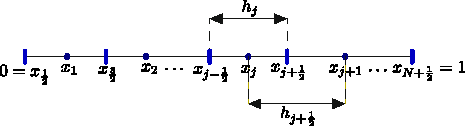
\includegraphics[width=.55\textwidth]{fv1d}
		\caption{Ilustración de una malla de volúmenes finitos
			unidimensional de $\Omega=\left(0,1\right)$.
			La malla contiene un conjunto de nodos de índices enteros
			\begin{math}
				{\big\{x_{j}\big\}}^{N}_{j=1}
			\end{math},
			que representan los puntos de aproximación, y otro conjunto de
			nodos de índices fraccionarios
			\begin{math}
				{\big\{x_{j+\tfrac{1}{2}}\big\}}^{N}_{j=1}
			\end{math}.
			\begin{math}
				x_{j}
			\end{math}
			es el centro de la celda
			\begin{math}
				\Omega_{j}=
				\big[
					x_{j-\tfrac{1}{2}},
					x_{j+\tfrac{1}{2}}
					\big]
			\end{math}
			cuyo tamaño es
			\begin{math}
				h_{j}=
				x_{j+\tfrac{1}{2}}-
				x_{j-\tfrac{1}{2}}
			\end{math}.
			La distancia entre dos celdas consecutivas es
			% \forall j=0,\dotsc,N:
			\begin{math}
				h_{j+\tfrac{1}{2}}=
				\frac{1}{2}\left(h_{j}+h_{j+1}\right)=
				x_{j+1}-x_{j}
			\end{math}.
		}
	\end{figure}
\end{frame}
